\chapter{Collaboration and Communication in Design} % Main chapter title

\label{Chapter6} % Change X to a consecutive number; for referencing this chapter elsewhere, use \ref{ChapterX}

\lhead{Chapter 6. \emph{Collaboration and Communication in Design}} % Change X to a consecutive number; this is for the header on each page - perhaps a shortened title


%----------------------------------------------------------------------------------------
%	NOTES
%----------------------------------------------------------------------------------------
\begin{comment}

The ultimate aim of the communication investigation was to establish communication types between building services consultants and contractors, and building services engineers and other stakeholders.

\section{Literature}

Finnish paper
\begin{figure}[htbp]
	\centering
	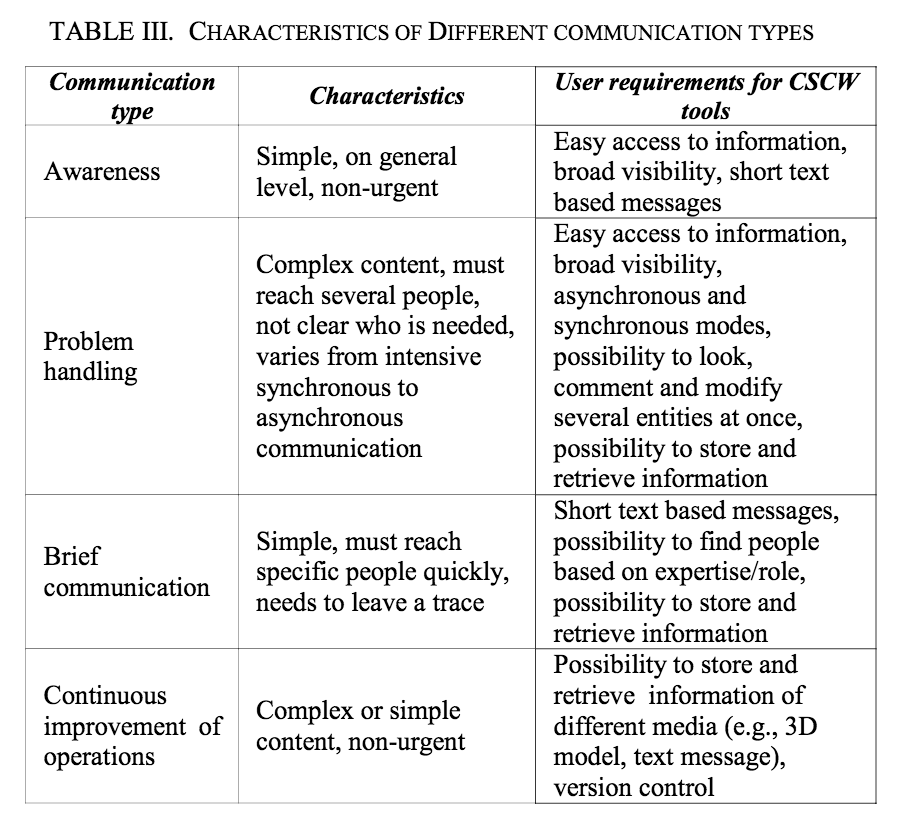
\includegraphics[width=.6\textwidth]{figures/Communication-types-table.png}
	\caption{Communication types}
	\label{comm_types}
\end{figure}

\textit{How designers think; the design process demystified}
(2nd ed. 1990)
by Bryan Lawson
\begin{itemize}
	\item Evolution of design:
	\begin{itemize}
		\item vernacular/ traditional design process
		\item cult of the individual (le Corbusier, Frank Lloyd Wright)
		\item ``collective control" (Jones), process forced to become more open to inspection and critical evaluation + scientific method
	\end{itemize}
	\item Jones' ``ultimate" definition of design: ``To initiate change in man-made things."
	\item Design process
	\begin{itemize}
		\item RIBA PoW is not a description of process, but of products of process
		\item ``It is about as much help in navigating a designer through his task as a diagram showing how to walk would be to a one year old child. [...] You will just have to put it all together for yourself." P. 28
	\end{itemize}
	\item Designing with others 
	\begin{itemize}
		\begin{figure}[htbp]
			\centering
			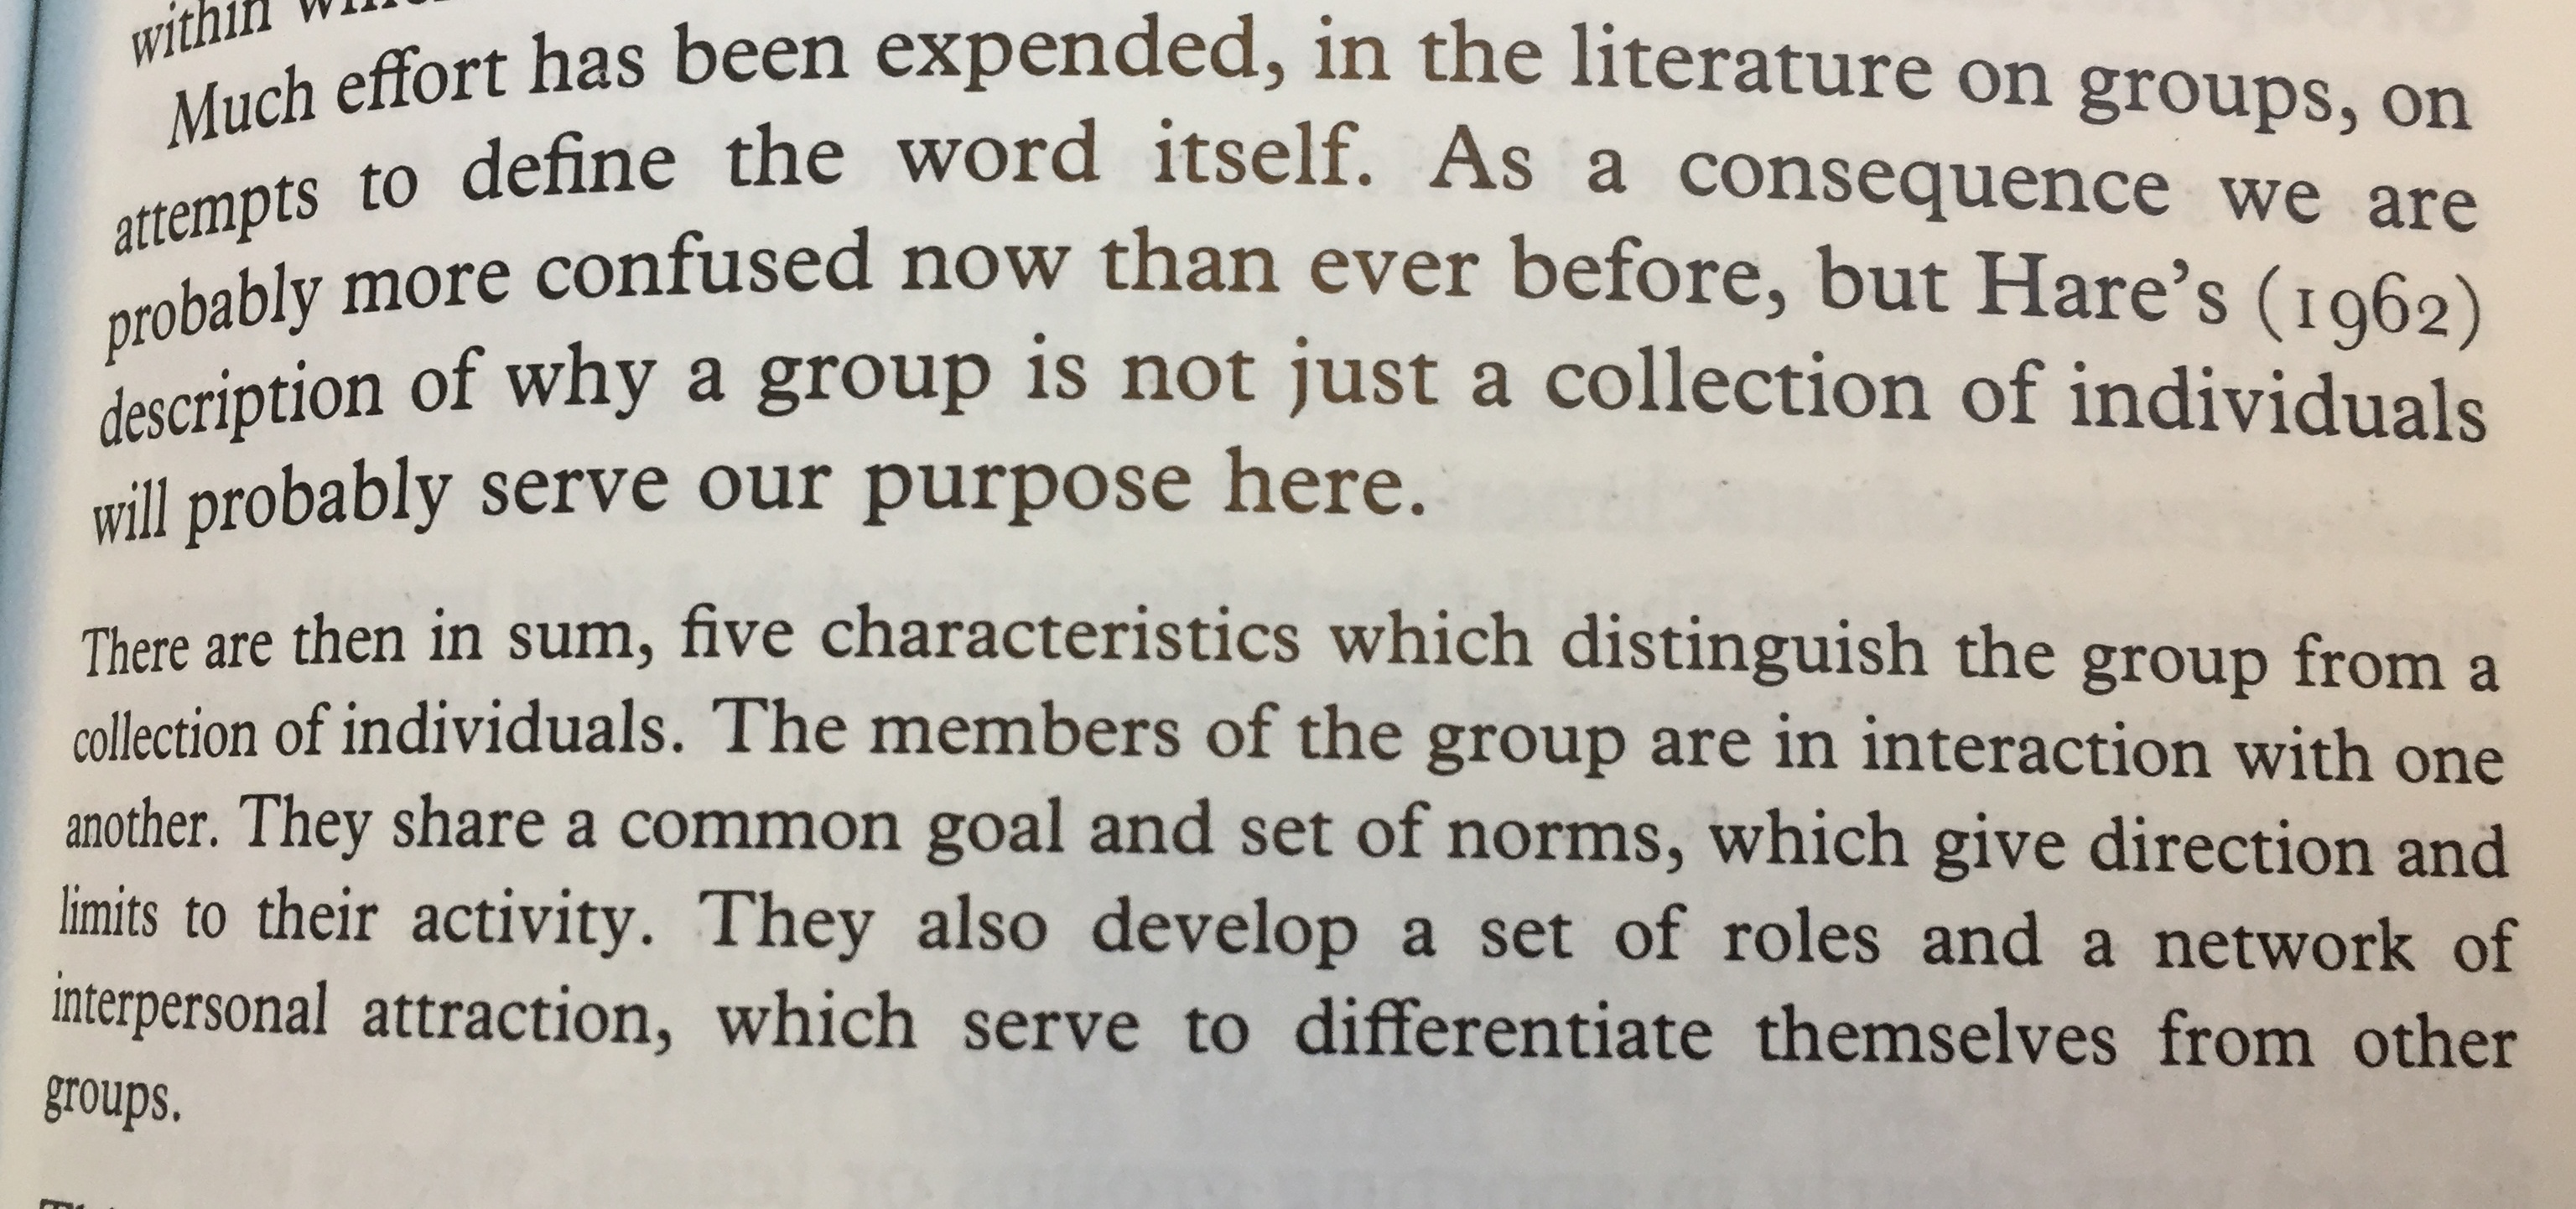
\includegraphics[width=.6\textwidth]{figures/Image.jpeg}
			\caption{Extract}
			\label{extract}
		\end{figure}
		\item Group vs. Collection of individuals - construction industry often acts as the latter? P. 189
		\item ``little has yet been written explicitly about design groups" p. 189
	\end{itemize}
\end{itemize}


\section{Interview}

	% title = {{MA PhD, Associate Professor at the School of Textiles \& Design at Heriot-Watt University}},

The purpose of the interview with Britta Kalkreuter was to find common language on describing communication in design.
This was to be done through hopefully drawing parallels between the construction and fashion industries.

Unfortunately, this comparative approach kind of backfired when I found out that Britta does not have much experience in fashion/ textiles.
She has a history in architectural history.
The courses she lectures at the School of Textiles and Design are primarily concerned with expression in the written word.
Her current research interests are in:
\begin{enumerate}
	\item Semantics and semiotics
	\item Design thinking and craft practice
	\item Heritage
\end{enumerate}
She described product semantics as \say{what a product communicates about itself or something else}.
My interests in communication might overlap with her interests in semantics and and design thinking.

The things we spoke about:
\begin{itemize}
	\item Design processes: crafts-based/ exploration of materials vs. designing for the end-user
	\item Modelling software
	\item Consultant/ contractor and designer/operator handover
	\begin{itemize}
		\item Communication breakdowns in designer/operator handovers
	\end{itemize}
	\item Communication 
	\begin{itemize}
		\item Her PhD student's paper - ``Craft and design interface", how negotiation occurs between craftsman and designer
		\item Communication types identified in Finnish journal article, particularly \say{continuous improvement of operations}
	\end{itemize}
\end{itemize}


%%%	EXCERPTS FROM INTERIM REPORT

The industry’s poor performance can largely be attributed to the its paradoxical nature; despite the in- dustry’s essence being intense collaborations on bespoke projects in temporary groupings (Laakso & Kiviniemi 2012), the industry is fragmented, with individual disciplines tending to work in isolation from others (IPA 2016, Miettinen & Paavola 2014).
--> WHY HAS COLLABORATION BEEN COUNTER-INTUITIVE TO CONSTRUCTION PROFESSIONALS WHEN IT IS REQUIRED?

The reports called for a reinvention of the AEC industry to improve its per- formance and put the client back in the centre. In order to achieve this, a need for collab- oration and standardisation was highlighted.
--> STDISATION FACILITATES/ ENABLES COLLABORATION

Amongst the government’s strategies for achieving this goal were enabling early contractor and supply chain involvement, standardising products and processes, and replacing adversarial cultures with collaborative ones. As part of the mobilisation towards collaboration, GCS 2011-15 required Building Information Modelling (BIM) Level 2 (explained in section 2.3) as a minimum on all public sector projects by 2016,
--> EARLY KOR INVOLVEMENT ALLOWS EARLIER COMMUNICATION + SMOOTHER HANDOVERS
--> IS THERE AN ADVERSARIAL CULTURE BETWEEN CIBSE AND TECHNICIANS/ WORKERS?
--> BIM INTRODUCED OUT OF NECESSITY FOR IMPROVED COLLABORATION

NBS (2014) defines BIM Level 2 as “distinguished by collaborative working –
all parties use their own 3D CAD models, but not necessarily working on a single, shared model. The collaboration comes in the form of how the information is exchanged between different parties – and is the crucial aspect of this level. Design information is shared through a common file format [such as IFC (Industry Foundation Classes) or COBie (Construction Operations Building Information Exchange)], which enables any organisation to be able to combine that data with their own in order to make a federated BIM model, and to carry
out interrogative checks on it.”
--> BIM LVL 2 DISTINGUISHED BY COLLABORATION THRU THE WAY INFO IS EXCHANGED (IFC, COBIE ETC.) --> DEFINITE BREAKDOWN IN COLLAB/ BIM LVL 2 WHEN IT COMES TO CONS TO KOR HANDOVER

\end{comment}

%----------------------------------------------------------------------------------------
%	INTRO
%----------------------------------------------------------------------------------------

% \hl{Alex: I would state that Egan, Latham, Collab4Change, even Farmer, all state collaboration / communication as a core issue and all as a positive contribution to effective performance. (Basically what you do at the start of Chapter 6)	That's enough.}

\cite{Latham1994}, \cite{Egan1998}, the government \citep{GCS11-15, GCS16-20} and \cite{Farmer2016} have all identified a lack of collaboration as being one of the great impediments to the effective performance of the AEC industry.
They have therefore asked AEC professionals to improve on their collaboration in order to deliver projects on time, on budget, and of good quality.
% The reports called for a reinvention of the AEC industry to improve its per- formance and put the client back in the centre. In order to achieve this, a need for collab- oration and standardisation was highlighted.
% So the industry/ government has asked the industry to get its sh*t/ act together and to start cooperating and collaborating better in order to provide better value, and reduce wastes in time and money.
This chapter will consider what is being asked of the industry by answering the following questions:
% Well, maybe we should delve into what is really being asked of the industry: 
\begin{enumerate}
	\item What is collaboration?
	% \item What does collaboration look like in the design and construction of a building?
	% \item Where and how does collaboration apply to building services engineers?
	\item What do collaboration and communication look like in the design and construction of a building?
	\item What are some failures in collaboration?
	% \item What should collaboration ideally look like in the setting…?
\end{enumerate}


%----------------------------------------------------------------------------------------
%	SECTION 1
%----------------------------------------------------------------------------------------

\section{What is Collaboration?}

\cite{collabor:oxford} defines collaboration as ``The action of working with someone to produce something".
\cite{wood1991toward} define collaboration as occurring ``when a group of autonomous stakeholders of a problem domain engage in an act or decide on issues related to that domain".
Further exploring the idea of a `group', according to \cite{hare1962handbook}, cited by \citeauthor{lawson1990} [\citeyear[p.~189]{lawson1990}], there are five characteristics that distinguish the group from a collection of individuals:
``The members of the group are [1] in interaction with one another.
They share [2] a common goal and [3] set of norms, which give direction and limits to their activity.
They also develop [4] a set of roles and [5] a network of interpersonal attraction, which serve to differentiate themselves from other groups."

Common traits that can be gathered from those three definitions are that collaboration is defined by:
\begin{itemize}
	\item Acting, deciding and/ or producing something %act, action, activity, decide, produce
	\item An interaction with at least one other person %with someone and group and interaction
	\item A shared problem and goal among the stakeholders %problem domain and common goal and set of norms
	\item The people involved each having an interest or concern in the problem or goal %autonomous roles
	\item The stakeholders being free to act independently
	\item The development of standard ways for the stakeholders to communicate with each other %and  (a person with an interest or concern in something (Oxford))
\end{itemize}



%----------------------------------------------------------------------------------------
%	SECTION 2
%----------------------------------------------------------------------------------------

\section{Collaboration and Communication in the Design and Construction of a Building}


%----------------------------
%	SUBSECTION 1
%----------------------------

\subsection{Where and How Does Collaboration Apply to Building Services Engineers?}

There are at least three different levels of communication and collaboration that building services engineers undergo during a project:
\begin{itemize}
	\item Discussion with the client/ employer about the end goal of the project (e.g. new build, refurbishment, expansion) and the issues related to achieving that goal.
	These times of discussion typically occur at the conceptual stage of a project and at planned checkpoints or meetings throughout the rest of the project.
	% Client/ employer, providing brief/ project requirements/ framework/ problem/ goal
	\item Communication and collaboration regarding the design and construction of the facility in the following settings:
	\begin{itemize}
		\item Discipline-external, i.e. with architects, structural engineers, project managers, quantity surveyors etc.
		\item Discipline-internal, i.e. with building services consultants and contractors etc.
	\end{itemize}
\end{itemize}

Processes, e.g. the RIBA PoW 2013, and contracts define the stages of a project and the required outputs of each stage.
It is important to note that processes such as the RIBA PoW 2013 are not prescriptive, but they merely provide a ``framework for the project team to approach design, construction and operational processes" \citep{Fairhead2015:online} by describing ``the products of the process" \citep{lawson1990}. % \hl{page number of quote} .
The reason for this is that the stakeholders, especially the designers, need freedom to act independently.
An analogy that explains designers' need of freedom from prescription is:
``It is about as much help in navigating a designer through his task as a diagram showing how to walk would be to a one year old child. [\ldots] You will just have to put it all together for yourself" \citep[p.~28]{lawson1990}.
Hence, one cannot say exactly when and with whom a building services engineer will collaborate; depending on the required outputs for each stage, building services engineers should seek collaboration with the appropriate people.
% Example: RIBA PoW 2013 “provides a framework for the project team to approach design, construction and opera- tional processes”
% + RIBA PoW is not a description of process (or is it?), but of products of process.


%----------------------------
%	SUBSECTION 2
%----------------------------

\subsection{Collaboration Patterns in Design}

% Despite this, it is worthy to note that t
The degree of collaboration between stakeholders on a design project has a typical pattern.
\cite{Parraguez2015} studied and identified patterns in the information flows between activities performed by stakeholders throughout the stages of complex engineering design projects.
They achieved this by analysing a ``large dataset collected from an industrial setting, consisting of project-related e-mails and activity records from the design and development of a renewable energy plant over the course of more than three years" \citep[p.~604]{Parraguez2015}.
They identified the stages of an engineering design process (see Figure \ref{fig_Parraguez_stages}) and three categories of design activities based on their functions.
``The first category includes activities related to the engineering design of specific components, modules, or subsystems under development; these we call modular subsystem activities.
The second category corresponds to activities with the objective of integrating two or more components, modules, or subsystems; these we call integrative subsystem activities.
A third category [\ldots] corresponds to activities that support, manage, and coordinate design work; for consistency, we call these integrative work activities" \citep[pp.~605--606]{Parraguez2015}.
% These three categories allow classifying activities based on their overall function and with this the means for aggregated analysis of information flows of each design stage."
The three categories allowed \citeauthor{Parraguez2015} to analyse the information flows between design activities  during each stage of the project.


\begin{figure}[tbp]
	\centering
	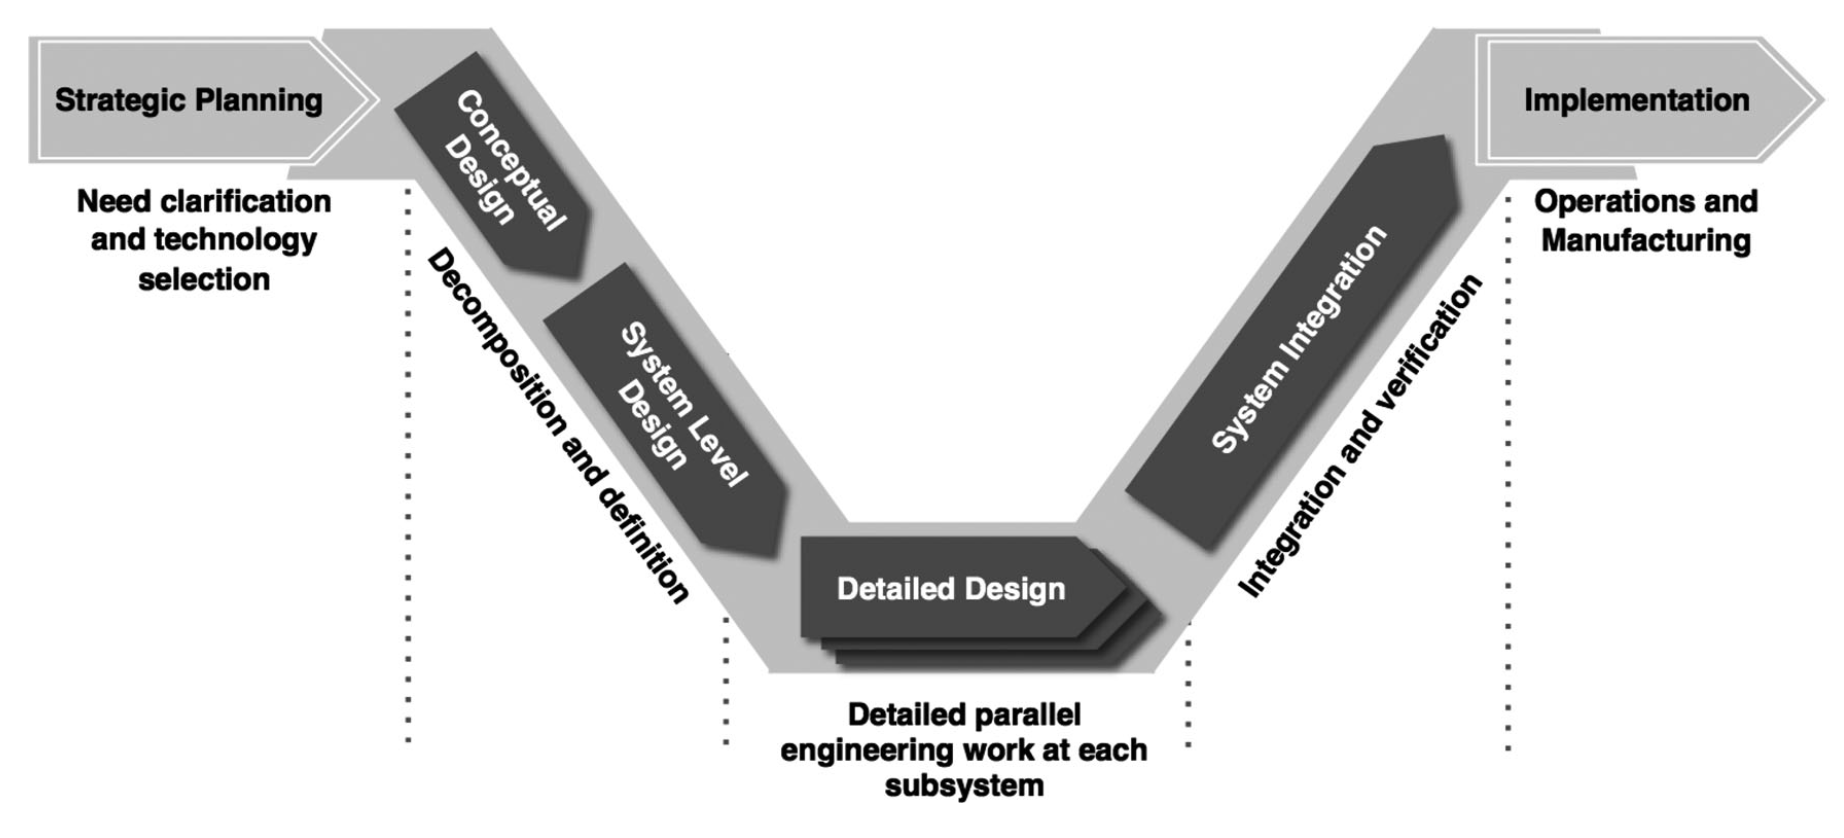
\includegraphics[width=\textwidth]{figures/Parraguez_stages.png}
	\rule{\textwidth}{0.5pt} % use line???
	\caption[Stages of the engineering design process.]{Stages of the engineering design process that can similarly apply to the stages of a building design process \citep[Figure~1]{Parraguez2015}.}
	\label{fig_Parraguez_stages}
\end{figure}


Figure \ref{fig_Parraguez_patterns} summarises their findings regarding the information patterns between activities for each stage.
% As illustrated in Figure \ref{fig_Parraguez_patterns} from \cite{Parraguez2015} who studied information flows in complex engineering design projects through activities and emails etc. (?).
It can be observed that there are strong information flows between and within most modular subsystem activities and integrative work activities at the Conceptual Design and System-Level Design stages.
However, at these early stages, the integrative subsystem activities and some of the modular subsystem activities have not yet established strong information flows within themselves.
At the Detailed Design stage, all of the activities have strong information flows within themselves, but there are weak information flows between the activities.
Lastly, at the System Integration stage, there are strong information flows within all activities and between most activities.
If the information flow patterns applied to the design process of a building, the findings of \cite{Parraguez2015} can be interpreted as follows:
\begin{enumerate}
	\item At the start of a project, there is strong collaboration between the client/ employer, designers and contractors in order to set and understand the brief; support, manage and coordinate the design work; and begin the individual design activities of the stakeholders.
	\item During the more detailed design stages, the stakeholders work mostly autonomously on modular subsystem activities with few interactions with each other.
	However, there might be strong collaboration between stakeholders on integrative subsystem activities.
	\item During the construction stage, there is strong collaboration between most activities.
\end{enumerate}

Regarding Stage 4 Technical Design, the RIBA PoW 2013 supports the second point:
``Using the design coordinated during the previous stage [i.e. Stage 3 Developed Design], the designers should now be able to develop their Technical Designs independently, with a degree of autonomy"
% The lead designer will provide input to certain aspects, including a review of each designer’s work" 
\citep{RIBAPlan}.


\begin{figure}[tbp]
	\centering
	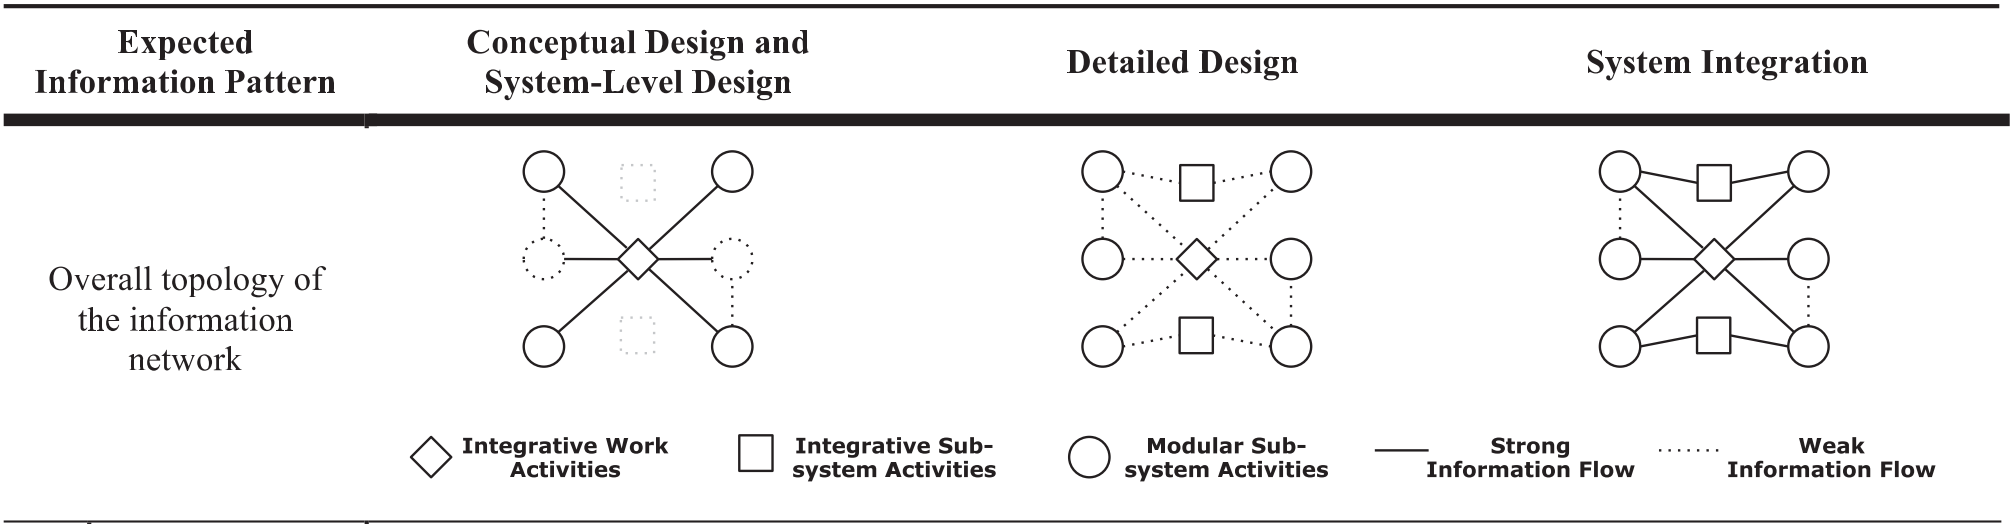
\includegraphics[width=\textwidth]{figures/Parraguez_patterns.png}
	\rule{\textwidth}{0.5pt} % use line???
	\caption[Information flow patterns between activities for each design stage.]{Information flow patterns between activities for each design stage \citep[Table~III]{Parraguez2015}.}
	\label{fig_Parraguez_patterns}
\end{figure}


%----------------------------
%	SUBSECTION 3
%----------------------------

\subsection{Communication Types in Design}

% \hl{Topic sentence.}
\cite{Holtta} studied and identified different types of communication regarding design content or design process in a buyer-supplier relationship within a product development network.
Additionally, \citeauthor{Holtta} highlighted characteristics of the design communication types that would facilitate the development of more effective communication tools.
They achieved this by studying the communication between a foundry\footnote{A foundry is a workshop or factory for casting metal \citep{foundry:oxford}.} and three of its customers, for whom the foundry manufactured components that were to be integrated with the customers' products.
A parallel could be drawn between this and the relationship that a product manufacturer or specialist designer has with a consultant.
Table \ref{table_communication_types} summarises their findings.
% \hlc{Create Latex table + explain then discuss findings (parallels to building design)}

% Please add the following required packages to your document preamble:
% \usepackage{booktabs}
\begin{table}[htbp]
\centering
\caption[Characteristics of different communication types.]{Characteristics of different communication types \citep[Table~III]{Holtta}. *CSCW: computer supported collaborative work.}
\label{table_communication_types}
\resizebox{\columnwidth}{!}{%
\begin{tabular}{@{}lll@{}}
	\toprule
	Communication type & Characteristics & User requirements for CSCW* tools \\ \midrule
	Awareness & \specialcell{l}{Simple, on general \\ level, non-urgent} & \specialcell{l}{Easy access to information, \\ broad visibility, short text \\ based messages} \\
	 & & \\
	Problem handling & \specialcell{l}{Complex content, must \\ reach several people, \\ not clear who is needed, \\varies from intensive \\ synchronous to \\asynchronous \\ communication} & \specialcell{l}{Easy access to information, \\ broad visibility, \\ asynchronous and \\ synchronous modes, \\ possibility to look, \\ comment and modify \\ several entities at once, \\ possibility to store and \\ retrieve information} \\
	 & & \\
	Brief communication & \specialcell{l}{Simple, must reach \\ specific people quickly, \\ needs to leave a trace} & \specialcell{l}{Short text based messages, \\ possibility to find people \\ based on expertise/ role, \\ possibility to store and \\ retrieve information} \\
	 & & \\
	\specialcell{l}{Continuous improvement \\ of operations} & \specialcell{l}{Complex or simple \\ content, non-urgent} & \specialcell{l}{Possibility to store and \\ retrieve information of \\ different media (e.g., 3D \\ model, text message), \\ version control} \\ \bottomrule
\end{tabular}
}
\end{table}


%----------------------------------------------------------------------------------------
%	SECTION 4
%----------------------------------------------------------------------------------------

\section{Communication \& Collaboration Failures}

% What are the weak points in collaboration/ why has the industry failed to collaborate so far/ why has collaboration been counter-intuitive to construction professionals when it is required?

Collaboration is often required in the AEC industry because the extent of a project can often exceed one's own knowledge and skill set.
However, information that is exchanged between multiple parties can be prone to distortion or even complete disappearance, such as in language translations and in the game \textit{Chinese Whispers}.

Communication failures seem to be a common problem when designing with others.
For example, in the fashion industry, labels that describe the materials used in an article of clothing are often inaccurate \citep{Kalkreuter2018}.
A designer may give a machine operator their design for a sweater in 100\% wool.
However the machine operator knows, through his practical craftsman skills, that it is impossible to weave wool in the way the designer has asked without adding nylon.
And so the machine operator adds nylon.
Along the way, the label may not get updated to state that the article contains both wool and nylon; instead, it states `100\% wool'.
This information may be left out accidentally or deliberately, perhaps because wool may be regarded as more valuable by the customer.
% \hl{listen to recording for jargon and re-write paragraph properly}.

% Common problem.
% Example: incorrect label problem during designer-manufacturer handover in textiles

% Idea of losing information during handovers, c.f. Chinese whispers, lost in translation?
% Can be researched further?
% Possible solution: minimise or eliminate handovers?
% Problem of skill set… Designer may not be able to manufacture and vice-versa.
% (That's the whole idea of collaboration and synergy, duh!)

% No regular meetings with client to understand goal.
% Famous chart where changes at the start are cheaper than changes towards the end of a project.
% Not fully understanding extent of project from outset.


%----------------------------------------------------------------------------------------
%	SECTION 5
%----------------------------------------------------------------------------------------

% \section{Conclusion/ Summary}
